\chapter{Industrial Process Control Domain Chapter}
\label{ch:domain-industrial}

Industrial process control is proof-validated within a bounded contract: real telemetry, verified training surfaces, replay closure, and material post-repair safety improvement all clear the current gate.

\section{{Domain problem}}
Industrial plants face thermal, pressure, and power safety constraints under unreliable sensor networks where stale or missing observations can hide excursions until they have already become operational hazards.

\section{{Degraded-observation hazard}}
The ORIUS book forces every domain through the same hazard lens: the runtime does not act
on the true state directly; it acts on a degraded, delayed, or otherwise imperfect
observation surface.  The row is only credible if the gap between those two surfaces can
be expressed, replayed, repaired, and audited explicitly.
The row stresses packet loss, stale reads, spikes, and out-of-order process measurements that mimic degraded plant telemetry rather than laboratory noise.

\section{{ORIUS instantiation}}
The industrial adapter reuses the universal kernel by swapping in process-specific state features, constraint evaluation, and action repair against the plant envelope.

\section{{Safety object}}
The defended predicate is zero true-state violation of the bounded process envelope after the repaired action is issued, while preserving plant continuity better than a brute shutdown response.

\section{{Dataset and training surface}}
The current surface uses the locked industrial telemetry row, the verified training audit, and the shared universal replay harness.
The chapter-local evidence packet is intentionally tied to locked artifacts rather than to
narrative memory.  Table~\ref{tab:ch40-44-cross-domain-support} gives the shared cross-domain
support layer for compiled Chapters~40--44, while the table below isolates the current row.

\section{{Feature, split, and training protocol}}
This chapter uses the verified split surface from the universal training audit. The current primary target is \texttt{power\_mw}, and the parity gate still records the raw/data surface as \texttt{verified} rather than as a prose-only claim.

\IfFileExists{paper/assets/tables/generated/tbl_industrial_training_surface.tex}{%
\begin{table}[htbp]
\centering
\small
\caption{Industrial Process Control training and data surface for the compiled chapter evidence block.}
\label{tab:industrial-training-surface}
\begin{tabular}{p{0.31\linewidth}p{0.61\linewidth}}
\toprule
\textbf{Field} & \textbf{Value}\\
\midrule
Raw/data gate & verified\\
Features present & yes\\
Split counts & train 6,680 / calibration 477 / validation 954 / test 1,433\\
Primary target & power\_mw\\
Forecast metrics & RMSE 3.609; MAE 2.729; PICP90 0.896; mean width 11.578\\
Verification state & split valid yes; model bundle yes; uncertainty yes; backtests yes\\
Artifact lineage & reports/orius\_framework\_proof/training\_audit/domain\_training\_summary.csv; reports/publication/orius\_equal\_domain\_parity\_matrix.csv\\
\bottomrule
\end{tabular}
\end{table}
%
}{%
\begin{table}[htbp]
\centering
\small
\caption{Industrial Process Control training and data surface for the compiled chapter evidence block.}
\label{tab:industrial-training-surface}
\begin{tabular}{p{0.31\linewidth}p{0.61\linewidth}}
\toprule
\textbf{Field} & \textbf{Value}\\
\midrule
Raw/data gate & verified\\
Features present & yes\\
Split counts & train 6,680 / calibration 477 / validation 954 / test 1,433\\
Primary target & power\_mw\\
Forecast metrics & RMSE 3.609; MAE 2.729; PICP90 0.896; mean width 11.578\\
Verification state & split valid yes; model bundle yes; uncertainty yes; backtests yes\\
Artifact lineage & reports/orius\_framework\_proof/training\_audit/domain\_training\_summary.csv; reports/publication/orius\_equal\_domain\_parity\_matrix.csv\\
\bottomrule
\end{tabular}
\end{table}
%
}

\section{{Replay and evidence surface}}
On the tracked evidence row, ORIUS reduces true-state violations from 21.53 percent to 0.00 percent, making industrial control one of the strongest non-battery demonstrations of universality in practice.

\IfFileExists{paper/assets/tables/generated/tbl_industrial_replay_surface.tex}{%
\begin{table}[htbp]
\centering
\small
\caption{Industrial Process Control replay, runtime, and promotion surface for the compiled chapter evidence block.}
\label{tab:industrial-replay-surface}
\begin{tabular}{p{0.31\linewidth}p{0.61\linewidth}}
\toprule
\textbf{Field} & \textbf{Value}\\
\midrule
Governing replay metric & baseline TSVR 21.53 -> ORIUS TSVR 0.00\\
Replay status & pass\\
Safe-action soundness & pass\\
Fallback semantics & power\_cap / bounded\_runtime\_pass\\
CertOS lifecycle & evaluated / evaluated\\
Paper 5 portability & evaluated / evaluated\\
Evidence tier & proof\_validated\\
Exact blocker & bounded\_to\_current\_plant\_family\\
Artifact lineage & reports/publication/orius\_domain\_closure\_matrix.csv; reports/universal\_orius\_validation/domain\_closure\_matrix.csv; reports/publication/orius\_equal\_domain\_parity\_matrix.csv\\
\bottomrule
\end{tabular}
\end{table}
%
}{%
\begin{table}[htbp]
\centering
\small
\caption{Industrial Process Control replay, runtime, and promotion surface for the compiled chapter evidence block.}
\label{tab:industrial-replay-surface}
\begin{tabular}{p{0.31\linewidth}p{0.61\linewidth}}
\toprule
\textbf{Field} & \textbf{Value}\\
\midrule
Governing replay metric & baseline TSVR 21.53 -> ORIUS TSVR 0.00\\
Replay status & pass\\
Safe-action soundness & pass\\
Fallback semantics & power\_cap / bounded\_runtime\_pass\\
CertOS lifecycle & evaluated / evaluated\\
Paper 5 portability & evaluated / evaluated\\
Evidence tier & proof\_validated\\
Exact blocker & bounded\_to\_current\_plant\_family\\
Artifact lineage & reports/publication/orius\_domain\_closure\_matrix.csv; reports/universal\_orius\_validation/domain\_closure\_matrix.csv; reports/publication/orius\_equal\_domain\_parity\_matrix.csv\\
\bottomrule
\end{tabular}
\end{table}
%
}

\begin{figure}[htbp]
\centering
\IfFileExists{reports/publication/fig_industrial_chapter_snapshot.png}{%
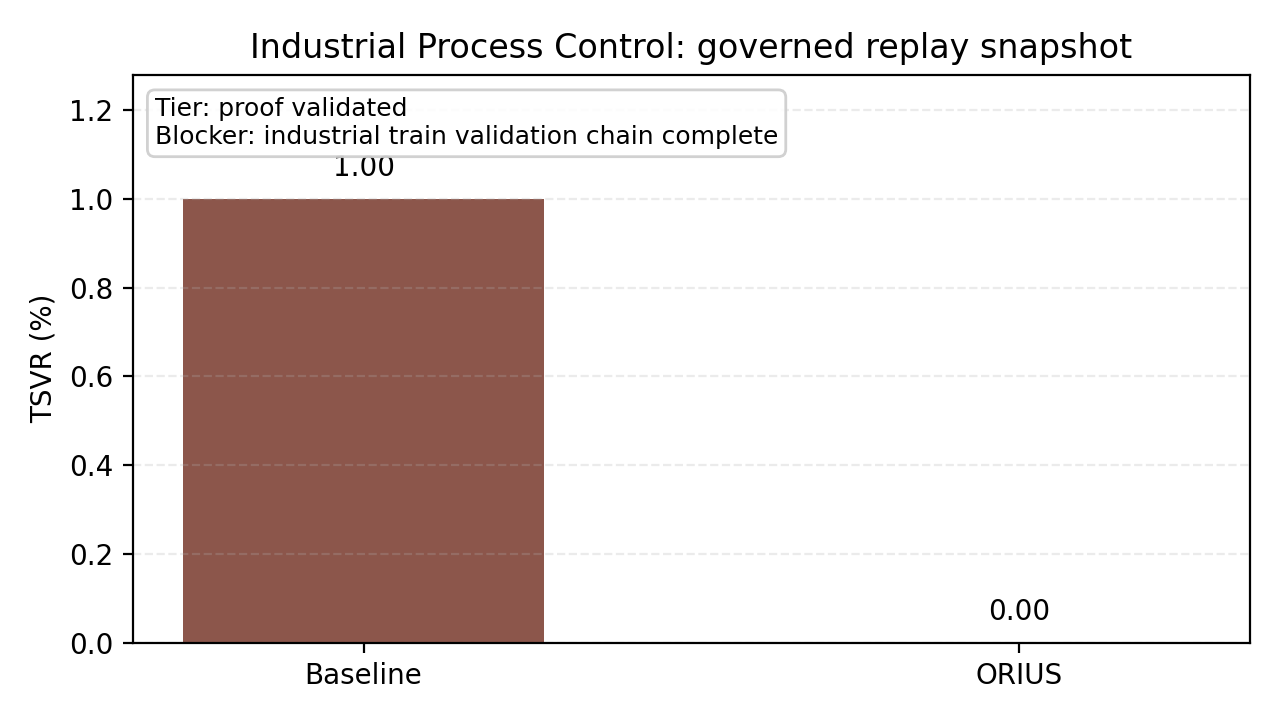
\includegraphics[width=0.90\textwidth]{reports/publication/fig_industrial_chapter_snapshot.png}%
}{%
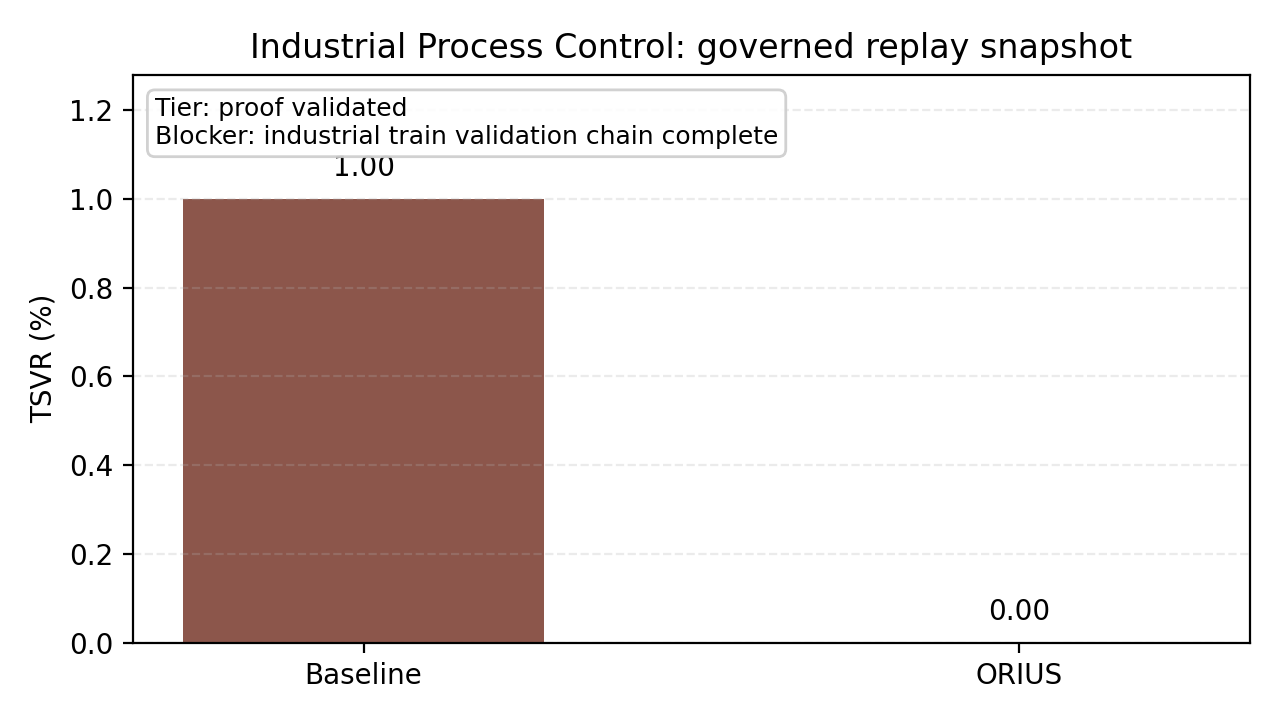
\includegraphics[width=0.90\textwidth]{../reports/publication/fig_industrial_chapter_snapshot.png}%
}
\caption{Industrial Process Control replay snapshot derived from the governed domain-closure artifact. Baseline and repaired TSVR are taken from the locked closure matrix; tier and blocker language remain governed by the parity gate.}
\label{fig:industrial-chapter-snapshot}
\end{figure}

\section{{Fallback and runtime behavior}}
Industrial control uses bounded power-cap and envelope-preserving fallback rather than brute shutdown, with CertOS lifecycle hooks recording every repaired or downgraded action.

\section{{Evidence tier and promotion blocker}}
The governing replay artifact for this row is the closure surface 1.0000 to 0.0000 TSVR transition under a replay status of pass. The evidence tier stays bounded by the parity gate rather than by narrative preference.



\section{{Limitations and exact non-claims}}
The proof-validated label is still bounded: the row is a defended domain instantiation, not a claim that every industrial control topology inherits the same guarantee automatically. This row does not claim every plant topology inherits the same guarantee automatically; it claims a defended bounded industrial envelope under the current replay and adapter contract.

The current promotion obligation for this row remains explicit: Future industrial extensions must retain real telemetry, replay closure, and explicit certificate semantics rather than relying on architecture-only analogies.
